\documentclass[a4paper,12pt,leqno]{article}

\usepackage{amssymb,amsmath,amsfonts}
\usepackage[a4paper,margin=2cm]{geometry}
\usepackage{newcent}
\usepackage[scaled=1.1]{newtxmath}
\usepackage{graphicx}
\graphicspath{{figures/}}
\usepackage[usenames,dvipsnames]{xcolor}
\usepackage{booktabs}
\usepackage{caption}
\usepackage{subcaption}
\newcommand{\fitwidetable}[1]{%
  \begingroup
  \setbox0=\hbox{#1}%
  \leavevmode
  \ifdim\wd0>\linewidth
    \resizebox{\linewidth}{!}{\box0}%
  \else\box0\fi
  \endgroup}

\providecommand{\tightlist}{%
  \setlength{\itemsep}{0pt}\setlength{\parskip}{0pt}}
\usepackage[pdfencoding=auto]{hyperref}

\usepackage[backend=biber, style=alphabetic]{biblatex}
\addbibresource{downscaling.bib}

% Empirical sections and tables use the screened release documented in
% paper/processing_review.json. Remaining TK items concern the wider paper.

\title{Where ERA5-Land Underestimates Temperature: A Pan-European,
Station-Level Diagnostic from GenHack'25}
\author{Saad So\underline{u}ilmi\footnote{TODO: confirm spelling/ordering of
author surname (GitHub handle is ``SaadSouilmi''; all three drafts wrote
``Soulimi'' -- please double check before submission).},
Imene Ben Rejeb-Mzah, Antoine Bezat, Anna Creti,\\
Charles-Albert Lehalle, Mengda Li, Gauthier Vermandel, Thomas Watteau}
\date{Printed the \today}

\begin{document}

\maketitle

\begin{abstract}
Gridded reanalysis fields provide spatially complete weather information,
but do not measure the same spatial footprint or necessarily the same
daily interval as station observations. Motivated by the GenHack'25
analyses, we compare ECA\&D daily maximum temperatures with supplied
ERA5-Land daily maxima across Europe. A conservative screening and
source-observation deduplication pipeline retains 6,958,414 station-days
at 4,217 nominal station IDs between January 2020 and August 2025.
The observation-weighted station-minus-reanalysis mean is
$1.58\,^\circ$C. Quantile-binned conditional means increase with station
temperature and decrease with the magnitude of the daily mean wind
vector. Elevation, coastal-distance and urban-class profiles are
non-monotonic; NDVI and the supplied precipitation proxy show smaller
variation. Joint bins have larger warm-temperature residuals under low
mean-vector wind. These are descriptive associations, with pointwise
station-bootstrap intervals, rather than causal effects or an
area-weighted estimate of European bias. Mixed observation windows,
provisional station screening, seasonal NDVI extrapolation and an
unresolved precipitation accumulation convention limit interpretation.
We discuss the implications for evaluating and developing downscaling models.

\end{abstract}

\paragraph{Acknowledgment to students.} Special thanks to all GenHack'25
participating teams, whose regional analyses and empirical insights are
the raw material of this paper, and in particular to the winning teams
[TK: list team names/affiliations]. We are also grateful to Kayrros for
technical support, infrastructure, and geospatial data provision, and to
\'Ecole Polytechnique for hosting the hackathon.

% ===========================================================================
\section{Introduction}
\label{sec:intro}

Gridded temperature products are widely used in climate econometrics,
energy-demand modelling, crop-yield estimation, exposure studies and
hydrology, often because local station coverage is sparse or gridded
fields are easier to merge with other spatial data. This substitution
requires an assessment of the difference between a grid-cell estimate
and a point measurement.

The product evaluated here is ERA5-Land, supplied on a
$0.1^\circ\times0.1^\circ$ grid. ERA5-Land replays the land component of
ERA5 with atmospheric forcing from ERA5. It does not directly assimilate
observations; observations influence it through that forcing.\footnote{\href{https://cds.climate.copernicus.eu/datasets/derived-era5-land-daily-statistics?tab=overview}{Copernicus ERA5-Land daily-statistics documentation}.}
Our pipeline compares supplied daily maxima against ECA\&D station
daily maxima; it does not evaluate a separately bias-adjusted Kayrros
temperature product or apply a new temperature downscaling model.

Surprisingly little is known about the spatial and statistical structure
of this error. A small number of studies have identified systematic
biases in mountainous terrain, where elevation and sub-grid orographic
variability degrade the match between the reanalysis grid cell and the
station it represents
\parencite{satyapragyan2026bias,sebbar2023ml_downscaling,jacobs2024filling,nogueira2022assessment,zou2022performance},
and in urban areas, where the urban heat island signal is only partially
resolved by the reanalysis grid
\parencite{jacobs2024filling,nogueira2022assessment,zou2022performance}.
These studies are regional and variable-specific: each identifies one or
two explanatory covariates (elevation, urban land cover) over one region,
and to our knowledge no study has, to date, mapped the ERA5-to-station
discrepancy jointly across the full set of plausible covariates
(temperature, precipitation, wind, distance to the sea, vegetation,
urbanisation class) at the scale of an entire continent. A systematic,
Europe-wide characterisation of \emph{where, when, and why} reanalysis
temperatures depart from station measurements has been missing.

The GenHack'25 hackathon at \'Ecole Polytechnique, with technical support
from Kayrros, offered a natural route to fill part of this gap.
Several hundred students, working in teams and given paired
station--product temperature data, were asked to identify the drivers of
the discrepancy. Because the problem decomposes naturally by region, most
teams produced analyses of geographically restricted subsets, using
heterogeneous -- and sometimes mutually inconsistent -- methodologies.
Individually, these projects vary in scope, method, and rigour, as is
expected from a hackathon. Collectively, however, they converged on a
recurring, cross-team narrative: the discrepancy is not noise, it has a
sign, and a handful of covariates recur as explanatory across very
different regions. This paper takes that collective observation
seriously. We do not report on individual team submissions; instead, we
recode the teams' findings into a single, consistent diagnostic pipeline
-- conditional mean residual by covariate bin, with
cluster-bootstrap confidence intervals resampled by station -- and re-run
it at the scale of the whole of Europe, rather than region by region, to
check which of the teams' regional findings hold up, and with what
strength, once pooled.

\paragraph{Contributions.}
\begin{enumerate}
    \item We assemble a harmonised European dataset of paired station and
    ERA5-Land daily maximum temperatures over 2020-01-01 to 2025-08-31,
    with 4,217 nominal station IDs and 6,958,414 screened station-days, together with geospatial covariates:
    elevation, distance to the sea, NDVI, DEGURBA urbanisation class,
    precipitation, and wind speed.
    \item We define the station--product residual and characterise its
    marginal and joint structure through quantile-binned conditional
    mean profiles, with cluster-bootstrap confidence intervals that
    account for within-station serial dependence
    (Section~\ref{sec:data}).
    \item We report, at pan-European scale, the marginal association
    between the residual and six covariates -- station temperature,
    precipitation, wind speed, NDVI, distance to the sea, and elevation
    -- together with a DEGURBA urbanisation breakdown
    (Section~\ref{sec:results}): a systematic underestimation by the
    ERA5-Land in the screened sample, larger residuals in joint high-temperature
    and low-wind bins, non-monotonic elevation and coastal profiles, and no more than a minor role for
    precipitation and vegetation at this scale.
    \item We document a temperature$\times$wind interaction whereby the
    warm-temperature residual is larger in low-wind bins
    than in high-wind bins, a result not, to our knowledge,
    previously reported at continental scale.
    \item We draw consequences for statistical and machine-learning
    downscaling, arguing that the residual structure documented here
    defines a natural target for bias-aware and residual-based
    downscaling models (Section~\ref{sec:discussion}).
\end{enumerate}

The full analysis pipeline is available as open-source code
\cite{souilmi_era5_resid_github} [TK: add Zenodo DOI if/when archived].

% ===========================================================================
\section{Related work}
\label{sec:related}

\subsection{Downscaling and rescaling: task definition}

Climate downscaling refers to the construction of local or
high-resolution climate information from coarse predictors. In the usual
supervised formulation, we observe a coarse atmospheric or land-surface
field \(x_L\) on a grid \(G_L\), optional high-resolution static or
dynamic covariates \(a_H\) on a finer grid \(G_H\), and a target field
\(y_H\) on \(G_H\). The target may be a regional climate model
simulation, a reanalysis product, a satellite product, or
station-interpolated observations. The learning problem is therefore not
merely image enlargement, but estimation of the conditional law
\[
    p(y_H \mid x_L, a_H, t, s),
\]
where \(t\) denotes time and seasonality and \(s\) denotes geographical
context. The coarse field should often be recoverable by applying a known
aggregation operator \(A\) to the high-resolution output, i.e.
\(A(y_H) \approx x_L\). This ``coarse consistency'' requirement
distinguishes climate downscaling from generic super-resolution and is
central when the output will be used for risk analysis, hydrology,
infrastructure planning, agriculture, or extreme-event attribution.

Two related but distinct tasks are commonly grouped under downscaling.
The first is \emph{statistical climate downscaling}: learning the
relationship between large-scale predictors and local climate
quantities, often with bias correction, quantile mapping, or weather
typing. The second is \emph{spatial super-resolution}: mapping a
low-resolution field to a high-resolution gridded field, frequently
conditioned on topography, land cover, vegetation indices, coast
distance, or surface radiative variables. Modern machine-learning papers
often combine both: they super-resolve a coarse field while also
correcting systematic biases and generating plausible small-scale
variability
\parencite{maraun2018statistical_downscaling,labeurthre2024overview_downscaling}.

The present paper is complementary to this literature: rather than
proposing a new downscaling method, we characterise the \emph{errors of
the supplied ERA5-Land product} that downstream studies routinely treat as
observations. In the language above, our object of study is the
discrepancy between the target \(y_H\) (station temperature) and the
reanalysis estimate \(\hat y_H\) over the station network.

\subsection{Documented biases between reanalysis and station temperature}
\label{sec:related-bias}

The idea that reanalysis temperature departs from station temperature in
a structured, covariate-dependent way is not new, but the existing
evidence is fragmented across a handful of region- and variable-specific
studies. In mountainous terrain, elevation and sub-grid topographic
heterogeneity have been repeatedly flagged as drivers of the discrepancy
\parencite{satyapragyan2026bias}, and terrain-aware downscaling work over
mountain regions shows that adding elevation-related covariates
materially improves the match to station data -- itself indirect evidence
that elevation is doing real explanatory work in the raw
reanalysis-station gap \parencite{sebbar2023ml_downscaling}. In cities,
several studies report that reanalysis products under-resolve the urban
heat island and that the resulting bias correlates with built-up land
cover or urbanisation intensity
\parencite{jacobs2024filling,nogueira2022assessment,zou2022performance}.
Beyond these two covariates, we are not aware of prior work that jointly
considers wind, precipitation, vegetation, and sea proximity as
explanatory variables for the same residual, nor of prior work that does
so at continental scale with quantified, station-clustered uncertainty --
which is the gap this paper addresses.

\subsection{Modern machine-learning downscaling for climate}
\label{sec:related-ml}

\subsubsection{From statistical models to deterministic deep learning}

Classical statistical methods remain important because they make the
assumptions of the task explicit. Linear or generalized linear transfer
functions, analog methods, quantile mapping, random forests, and other
machine-learning regressors link local climate variables to large-scale
circulation and surface predictors. They are comparatively interpretable
and inexpensive, but their success depends on stationarity assumptions:
the relation learned from historical data must remain valid under future
climate states. Their treatment of spatial coherence and extremes is also
limited unless explicitly modelled. For instance, recent applications to
ERA5-Land temperature over mountains show that adding terrain-aware
covariates can substantially improve local predictions, while also
exposing the sensitivity of downscaling errors to elevation and surface
heterogeneity \parencite{sebbar2023ml_downscaling}. Broader evaluations of
statistical downscaling for climate projections similarly emphasize that
no single method dominates across variables, seasons, regions, and
extreme-event metrics
\parencite{hernanz2022statistical_downscaling,tabari2021downscaling_drought}.

Deep learning reframes downscaling as a representation-learning problem.
Early super-resolution approaches such as DeepSD adapted convolutional
neural networks to climate grids, learning an end-to-end map from coarse
fields and auxiliary topographic information to high-resolution
precipitation or temperature \parencite{vandal2017deepsd}. U-Net,
residual networks, dense blocks, and encoder-decoder architectures then
became natural choices because they mix large-scale context with local
detail. These deterministic networks are strong baselines: they are fast
at inference time, easy to train with mean-square or mean-absolute
losses, and often improve RMSE and MAE. However, regression losses
encourage conditional averages. The resulting fields may look smooth,
understate extremes, and lose fine-scale spectral power even when
pointwise scores are good. This is a key limitation for climate-risk
applications, where the distribution and spatial organization of rare
events matter as much as the conditional mean.

\subsubsection{Attention mechanisms and auxiliary geospatial information}

Attention mechanisms address a specific weakness of plain convolutional
downscalers: not all covariates are equally informative everywhere. In
land surface temperature downscaling, for example, vegetation, water,
built-up area, slope, aspect, and surface reflectance may explain
different parts of the temperature signal depending on season and local
geography. The Attention Mechanism U-Net (AMUN) of
\textcite{li2025attention_downscaling} is a useful example. The method
uses Google Earth Engine to assemble ERA5-Land LST and seven
high-resolution auxiliary factors over China, then learns to downscale
hourly monthly-mean LST from \(0.1^\circ\) to \(0.01^\circ\). Its Global
Multi-Factor Cross-Attention module recalibrates the interaction between
coarse LST and auxiliary features; a feature-fusion residual dense block
extracts multilevel LST features; and a U-Net decoder reconstructs the
fine field. In simulated and real experiments, the model reports
substantially lower RMSE than a random-forest baseline.

This line of work is relevant beyond LST because it points to a general
design principle: downscaling models should learn \emph{where} and
\emph{when} to trust each explanatory variable. Orography may dominate
mountain temperature gradients, NDVI and land cover may dominate surface
heat contrasts, and large-scale humidity and winds may control
precipitation organization. Attention layers, cross-attention between
low-resolution climate states and high-resolution covariate maps, and
channel-wise gating are therefore natural tools for geophysical
downscaling. Their limitation is that they typically produce a single
best estimate unless combined with a probabilistic output layer or a
generative model. Our own diagnostic (Section~\ref{sec:results}) can be
read as the descriptive counterpart to this design principle: before
choosing which covariates a downscaling network should attend to, one
should establish which covariates actually correlate with the raw
reanalysis-station gap, and by how much -- which is exactly what the
partial-dependence analysis below provides.

\subsubsection{Generative downscaling: GANs, diffusion, and consistency
models}

Generative models are attractive for climate downscaling because the
target is intrinsically one-to-many. A coarse grid cell can correspond to
many plausible fine-scale temperature or precipitation patterns.
Conditional generative adversarial networks (GANs) were among the first
deep generative approaches used for climate and weather super-resolution.
They can sharpen fields and recover small-scale structure; examples
include adversarial super-resolution of wind and solar fields
\parencite{stengel2020adversarial_super_resolution}, precipitation
forecast correction and downscaling with CorrectorGAN
\parencite{price2022correctorgan}, and physically constrained GANs for
precipitation fields \parencite{hess2022physically_constrained_gan}. Their
drawbacks are familiar: adversarial training may be unstable,
probabilistic calibration is difficult, and physically meaningful
constraints must be added carefully.

Diffusion and score-based models provide a more explicit probabilistic
framework. Denoising diffusion models learn to reverse a noising process,
while score-based stochastic differential equation formulations learn a
time-dependent score field that transports noise into data
\parencite{ho2020ddpm,song2021score_sde}. In conditional downscaling, the
model samples \(y_H\) from noise while conditioning on \(x_L\), static
covariates, and possibly an initial deterministic estimate. The study
\emph{Generative Diffusion-based Downscaling for Climate} demonstrates
this idea in an idealized ERA5 experiment, recovering \(0.25^\circ\)
fields from \(2^\circ\) inputs and showing better fine-scale accuracy
than a standard U-Net, especially in spectral diagnostics
\parencite{watt2024diffusion_downscaling}. This is important because
spectral performance measures whether the model restores the spatial
scales that interpolation and deterministic regression tend to erase.

Recent diffusion papers also explore efficiency and physical realism.
Latent diffusion reduces computational cost by operating in a compressed
representation; \textcite{tomasi2025latent_diffusion_downscaling} use
this strategy to mimic kilometer-scale COSMO5.0\_CLM9 regional climate
simulations, asking whether AI can approximate aspects of dynamical
downscaling. Residual corrective diffusion models decompose the problem
into a deterministic mean prediction followed by a diffusion model for
the residual. This is the idea behind CorrDiff, which downscales
\(25\,\mathrm{km}\) reanalysis inputs to \(2\,\mathrm{km}\) regional
weather-model outputs over Taiwan, sharpening fronts and typhoons while
recovering realistic spectra and distributions
\parencite{mardani2025corrdiff}. A related direction replaces long
diffusion sampling chains with consistency models, which can generate
high-resolution samples in fewer steps. \textcite{hess2025consistency_downscaling}
show that such models can perform fast, scale-adaptive, uncertainty-aware
ESM downscaling and can generalize across Earth system model inputs
without retraining.

\subsubsection{Flow matching as an emerging alternative}

Flow matching is a recent generative paradigm that learns a
continuous-time velocity field transporting a simple base distribution
into the data distribution \parencite{lipman2023flow_matching}. For
downscaling, it has two attractive features. First, inference can be
formulated as solving an ordinary differential equation rather than
running many stochastic denoising steps, which may reduce sampling cost.
Second, physical constraints such as re-aggregation consistency, water
conservation, or humidity bounds can be expressed as penalties or
projection steps along the learned flow.

The first climate and weather applications are appearing quickly. A 2026
study uses residual flow matching to super-resolve coarse-resolution
weather forecasts, training only on reanalysis data and evaluating
whether re-coarsened outputs remain consistent with the original forecast
trajectory \parencite{delefosse2026flow_matching_weather}. Another 2026
study proposes physics-constrained adaptive flow matching for climate
downscaling, adding soft conservation constraints for precipitation and
humidity and evaluating a \(63\,\mathrm{km}\) to \(6.3\,\mathrm{km}\)
Central Europe task across multiple variables
\parencite{debeire2026physics_constrained_flow_matching}. These papers are
new, but they suggest that flow matching may be a useful successor or
complement to diffusion when fast sampling, ensemble generation, and
physical consistency must be balanced.

\subsubsection{Positioning of the present paper}
\label{sec:related-diagnostics}

The literature reviewed above is almost entirely \emph{corrective}: it
asks how to build a model that maps ERA5 (or another coarse field) onto
station-quality temperature. It is largely silent on the simpler, prior,
\emph{descriptive} question that motivates this paper: where and under
what conditions is the raw reanalysis-station gap largest, and which
easily available covariates predict it? Answering that question well is
what determines, in practice, which covariates a downscaling network such
as AMUN should be given, and where a residual-diffusion or
flow-matching correction such as CorrDiff is likely to matter most. To
our knowledge, no prior work provides a unified, Europe-wide,
covariate-level diagnostic of station--reanalysis residuals with
uncertainty quantification that accounts for within-station dependence;
we view the two literatures as complementary, with this paper
supplying the covariate-level diagnosis that the downscaling literature
currently takes largely as given.

% ===========================================================================
\section{Data, hackathon design, and methodology}
\label{sec:data}

\subsection{The GenHack'25 hackathon}

% TODO (Saad): confirm exact numbers (participants, teams, regions,
% dates) and add them here.
GenHack'25 was organised at \'Ecole Polytechnique, with Kayrros
providing technical support on data access and the geospatial processing
pipeline. Several hundred students, organised in teams, were given a
common task: identify and characterise the discrepancy between ERA5 2m
temperature and co-located weather-station observations. Teams were free
to choose their region of interest and their modelling approach; in
practice, most teams focused on a specific European country or
sub-region rather than on the continent as a whole. This paper does not
report on individual team submissions; instead, it distils the
covariates that recurred as explanatory across teams into a single,
consistent pipeline, and re-runs that pipeline over the whole of the
teams' combined domain, i.e.\ continental Europe.

\subsection{Data}

The screened release contains 6,958,414 station-day pairs at 4,217 nominal
station IDs, from 2020-01-01 to 2025-08-31. It retains the original
observation-day window metadata; these figures use the main sample with
mixed windows, rather than the separate UTC-window subset.

\begin{itemize}
\item \textbf{Target.} ECA\&D daily maximum air temperature, validated
against the source TX values and their quality flags.
\item \textbf{Reference.} Supplied ERA5-Land daily maximum 2m temperature
at the matched grid cell. Matches requiring a substituted land cell,
or a different grid cell at the actual observation source, are excluded.
\item \textbf{Residual.} $r_{it}=T^{\mathrm{station}}_{it}-T^{\mathrm{ERA5}}_{it}$;
a positive residual means ERA5-Land is cooler than the station.
\item \textbf{Covariates.} Station temperature, the supplied precipitation
proxy in metres, the magnitude of the daily mean wind vector (m/s),
NDVI, distance to the sea (km), elevation (m), and DEGURBA urbanisation
class. Geographical covariates refer to the actual observation source.
The precipitation proxy is not an established daily total.
\end{itemize}

\paragraph{Temperature screening and provenance.}
The raw matched input contains 10,467,039 observations at 6,064 nominal
station IDs. Removing rows outside the supplied ERA5-Land grid footprint
leaves 10,024,790 observations. Station temperatures are checked against
TX/10 with $\mathrm{Q\_TX}=0$, and ERA5-Land temperatures are converted
from Kelvin by subtracting 273.15. Saved temperature, wind and precipitation
values were checked against all supplied in-grid daily files; the recorded
check covers 10,024,790 station-days with no extraction mismatches.
This verifies extraction and arithmetic, not the instruments or upstream
aggregation.

Screening uses unique source-days at source coordinates. A value is flagged
if it is outside $[-60,50]\,^\circ$C; if it lies more than $20\,^\circ$C
above both, or below both, adjacent calendar days; or if it differs by
more than $20\,^\circ$C from the median of at least three same-day
neighbour observations. The spatial check considers up to ten distinct
locations among the 64 nearest candidates, 15--100 km away and within
300 m elevation. A missing neighbour comparison is not a passed check.
The rules flag 313 unique source-days. Every nominal station series that
uses a flagged source is quarantined, giving 55 quarantined station IDs.
These are provisional screening thresholds, not a calibrated quality-control
algorithm or proof that all excluded readings are erroneous.

The subsequent exclusions are applied in the order shown in
Table~\ref{tab:cleaning-selection}. Each retained $(\mathrm{SOUID},t)$
appears once, keeping the smallest eligible nominal station ID. No row
is selected by the size of its ERA5 residual. ECA\&D blended records can
borrow observations from nearby sources; a nominal station ID therefore
does not always identify the instrument that made the observation.\footnote{\href{https://www.ecad.eu/dailydata/datadictionary.php}{ECA\&D data dictionary on blended series}.}
The supplied participant-source metadata requires an inferred identifier
offset of $+100000$, while synoptic identifiers match directly. The raw
and matched identifiers are retained and ambiguous matches fail; provider
confirmation of this convention remains desirable.

\begin{table}[htbp]
\centering
\small
\caption{Sequential selection. Counts removed at each step refer only to rows surviving preceding steps.}
\label{tab:cleaning-selection}
\fitwidetable{%
\begin{tabular}{lrr}
\toprule
Step & Removed & Remaining \\
\midrule
Raw matched input & 0 & 10,467,039 \\
Outside grid footprint & 442,249 & 10,024,790 \\
Substituted land cell & 948,022 & 9,076,768 \\
Quarantined station series & 72,993 & 9,003,775 \\
Invalid observation source & 0 & 9,003,775 \\
Source-location grid mismatch & 1,093,595 & 7,910,180 \\
Repeated source-day & 951,766 & 6,958,414 \\
\bottomrule
\end{tabular}}
\end{table}


\paragraph{Observation windows.}
ERA5-Land daily maxima are maxima of hourly samples. ECA\&D observation
windows and measurement frequencies vary by source; matching calendar
dates does not make those sampling schemes identical. The main sample
retains the source-window labels. The separate UTC-window subset contains
3,528,147 observations at 2,154 nominal IDs, restricted to the supplied
TX3/TX21 metadata codes; it is not the sample used in the figures.

\paragraph{Covariates and missingness.}
Elevation, NDVI, DEGURBA and coastal distance refer to the observation
source, whose location may change within a nominal station series.
Country labels in Table~\ref{tab:desc_country_top10} and the map positions
refer to nominal station metadata. Each figure retains finite values for
its own covariates; no global complete-case filter is applied.

NDVI is sampled from the raster covering the actual season when present.
If a season is unavailable, the latest earlier raster from the same season
is carried forward, with raster dates, filename and lag retained.
Raster codes 0--254 are mapped to $[-1,1]$; nodata remains missing.
Of the retained observations, 4,927,797 have observed-season NDVI,
1,873,268 have extrapolated NDVI, and 157,349 have no usable NDVI.
This is an explicit seasonal extrapolation assumption, not measured
vegetation for the missing dates or a claim of exact periodicity.

DEGURBA uses the fixed 2020 GHS-SMOD classification, sampled in the raster's
coordinate system. Elevation is taken from source metadata; the sentinel
codes $-999$ and $-9999$ are treated as missing, leaving 3,825 observations
without valid elevation. Coastal distance uses the Natural Earth 1:10
million ocean coastline with the Caspian ring excluded. A nearest point
is selected in EPSG:3035 and its WGS84 geodesic distance is calculated;
the generalized coastline and projection make this an approximate covariate.

Wind is $\sqrt{\overline{u}_{10}^{\,2}+\overline{v}_{10}^{\,2}}$, using
the daily mean components. It is not the mean of hourly speed magnitudes.
Precipitation is the supplied daily-mean proxy in metres. Its upstream
accumulation recipe is unresolved, so no conversion to a daily total or
to mm/day is made.

\begin{table}[htbp]
\centering
\small
\caption{Continuous variables in the screened sample. Missing counts include nonfinite and invalid elevation values. Temperatures are in degrees Celsius, wind is the magnitude of the daily mean vector (m/s), and precipitation is a proxy in metres.}
\label{tab:desc_continuous}
\fitwidetable{%
\begin{tabular}{lrrrrrrrr}
\toprule
Variable & Missing & Mean & SD & P05 & P25 & P50 & P75 & P95 \\
\midrule
station\_celsius & 0 & 15.7 & 10 & -0.6 & 8.7 & 15.9 & 23 & 32 \\
era5\_celsius & 0 & 14.2 & 9.77 & -1.76 & 7.48 & 14.4 & 21 & 30.1 \\
residual & 0 & 1.58 & 2.49 & -2.13 & 0.26 & 1.44 & 2.78 & 5.83 \\
wind & 0 & 2.06 & 1.51 & 0.332 & 0.956 & 1.73 & 2.78 & 4.92 \\
tp & 0 & 0.00137 & 0.00287 & 1.64e-07 & 1.32e-05 & 0.00024 & 0.00139 & 0.00657 \\
dist\_to\_sea\_km & 0 & 138 & 138 & 1.43 & 27.1 & 90.6 & 216 & 412 \\
elevation & 3,825 & 399 & 437 & 6 & 84 & 251 & 597 & 1.21e+03 \\
ndvi & 157,349 & 0.414 & 0.226 & 0.00787 & 0.252 & 0.433 & 0.591 & 0.748 \\
\bottomrule
\end{tabular}}
\end{table}

\begin{table}[htbp]
\centering
\small
\caption{DEGURBA coverage in the screened sample. A nominal station ID may occur in more than one class when its observation source changes.}
\label{tab:desc_degurba}
\fitwidetable{%
\begin{tabular}{lrrrrr}
\toprule
Code & Class & Observations & Obs. (\%) & Station IDs & IDs (\%) \\
\midrule
10 & Water & 31,337 & 0.5 & 17 & 0.4 \\
11 & Very low density rural & 2,532,936 & 36.4 & 1,641 & 38.9 \\
12 & Low density rural & 2,205,318 & 31.7 & 1,314 & 31.2 \\
13 & Rural cluster & 537,064 & 7.7 & 338 & 8.0 \\
21 & Suburban & 712,167 & 10.2 & 433 & 10.3 \\
22 & Semi-dense urban cluster & 102,984 & 1.5 & 66 & 1.6 \\
23 & Dense urban cluster & 320,232 & 4.6 & 227 & 5.4 \\
30 & Urban centre & 516,376 & 7.4 & 312 & 7.4 \\
\bottomrule
\end{tabular}}
\end{table}

\begin{table}[htbp]
\centering
\footnotesize
\setlength{\tabcolsep}{4pt}
\captionsetup{font=footnotesize,skip=4pt,width=0.8\linewidth}
\caption{Top ten countries by nominal station count; percentages refer to the full screened sample.}
\label{tab:desc_country_top10}
\fitwidetable{%
\begin{tabular}{lrrrr}
\toprule
Country & Observations & Obs. (\%) & Station IDs & IDs (\%) \\
\midrule
Italy & 1,051,991 & 15.1 & 897 & 21.3 \\
Spain & 1,550,587 & 22.3 & 816 & 19.4 \\
Germany & 925,351 & 13.3 & 460 & 10.9 \\
Norway & 704,611 & 10.1 & 424 & 10.1 \\
Austria & 547,504 & 7.9 & 391 & 9.3 \\
Sweden & 420,909 & 6.0 & 217 & 5.1 \\
Finland & 312,269 & 4.5 & 159 & 3.8 \\
Hungary & 261,359 & 3.8 & 144 & 3.4 \\
Poland & 204,949 & 2.9 & 112 & 2.7 \\
Türkiye & 162,925 & 2.3 & 87 & 2.1 \\
\bottomrule
\end{tabular}}
\end{table}

\begin{table}[htbp]
\centering
\small
\caption{Screened temperature-pair sample; each figure uses available values for its own covariates.}
\label{tab:data-summary}
\fitwidetable{%
\begin{tabular}{lr}
\toprule
Quantity & Value \\
\midrule
Nominal station IDs & 4,217 \\
Station-days & 6,958,414 \\
Time period & 2020-01-01 to 2025-08-31 \\
Countries covered & 34 \\
Residual mean (SD), $^\circ$C & 1.58 (2.49) \\
\bottomrule
\end{tabular}}
\end{table}


\subsection{Methodology}
\label{sec:methods}

\paragraph{Covariate profiles.} For each covariate $X_j$, we estimate the
conditional mean residual $\mathbb{E}[r\mid X_j]$ using ten quantile bins,
merging duplicate boundaries. Means give each observation equal weight.
Points are plotted at bin midpoints, with outer bins bounded by observed
extrema. These are univariate descriptive profiles, not partial dependence
from a fitted multivariate model. The lower panels show histograms of
4,999 sampled observations, rather than the complete sample counts.

\paragraph{Inference.} Pointwise 95\% percentile intervals use $B=1000$
bootstrap resamples of nominal station IDs within each bin or class,
retaining all observations from each selected station. The seed is 1337,
and station groups are sorted before resampling. This accounts for
dependence within a station, but not dependence between nearby stations.
The intervals are neither simultaneous bands nor formal tests of the
differences between bins.

\paragraph{Joint profiles.} The temperature$\times$wind figure uses an
eight-by-eight grid of marginal quantile bins, with observation-weighted
mean residuals in each joint cell. It displays no confidence intervals
and does not estimate a causal interaction. Marginal histograms each use
4,999 sampled observations. Wind is the magnitude of the daily mean
vector, which is distinct from the daily mean wind speed.

% ===========================================================================
\section{Results}
\label{sec:results}

\subsection{ERA5-Land maxima are lower on average in the screened sample}
\label{sec:results-map}

\begin{figure}[htbp]
\centering
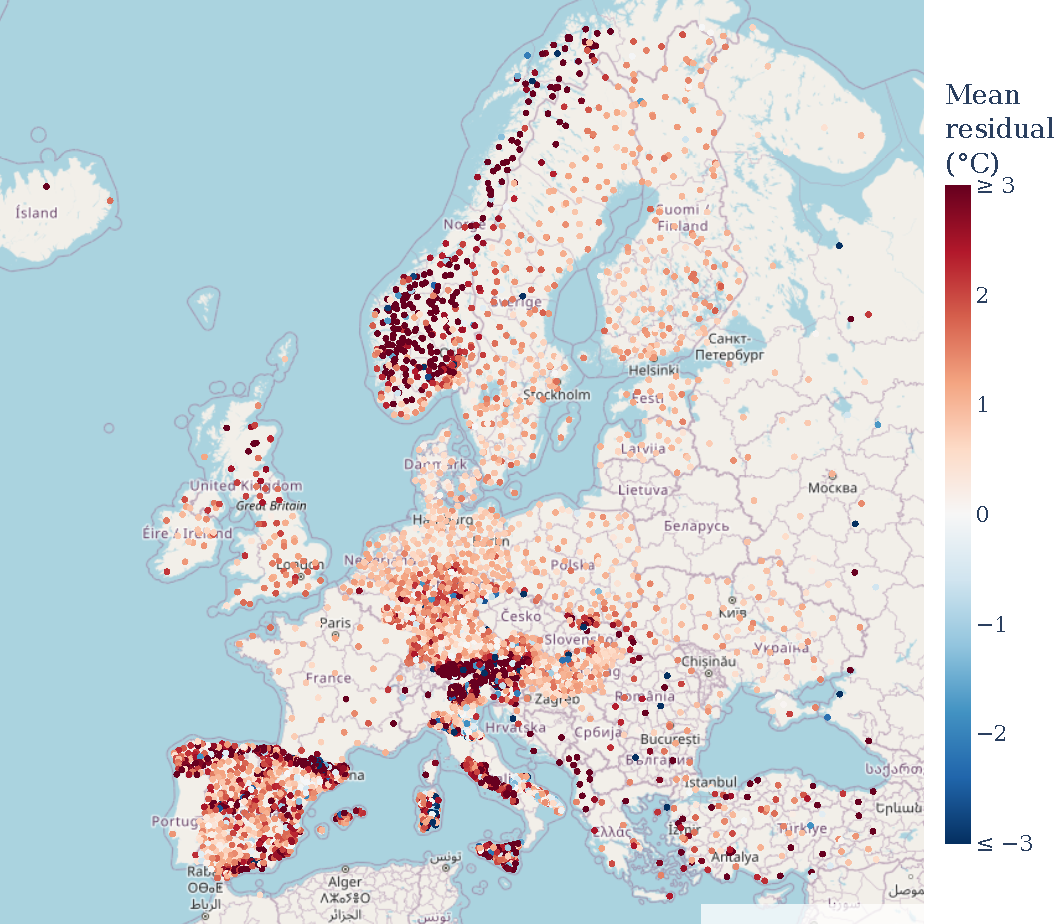
\includegraphics[width=\textwidth]{figures/station_map.pdf}
\caption{Mean station-minus-ERA5-Land residual at each nominal station ID,
all dates pooled. Positive (red) values indicate cooler ERA5-Land maxima.
Nominal station coordinates are used; the sources contributing to each
mean may change over time. All 4,217 IDs lie in the displayed window. Colours
saturate beyond $\pm3\,^\circ$C. Plotly map with an OpenStreetMap basemap
(\copyright\ OpenStreetMap contributors).}
\label{fig:map}
\end{figure}

The observation-weighted mean residual is $1.58\,^\circ$C; the mean
giving equal weight to each nominal station is $1.55\,^\circ$C.
Approximately 89.1\% of stations have a positive mean residual
(Figure~\ref{fig:map}). These quantities describe the screened station
sample, not an area-weighted European temperature bias.

\subsection{Residuals increase across station-temperature bins}
\label{sec:results-temperature}

\begin{figure}[htbp]
\centering
\begin{subfigure}[t]{0.32\textwidth}
\centering
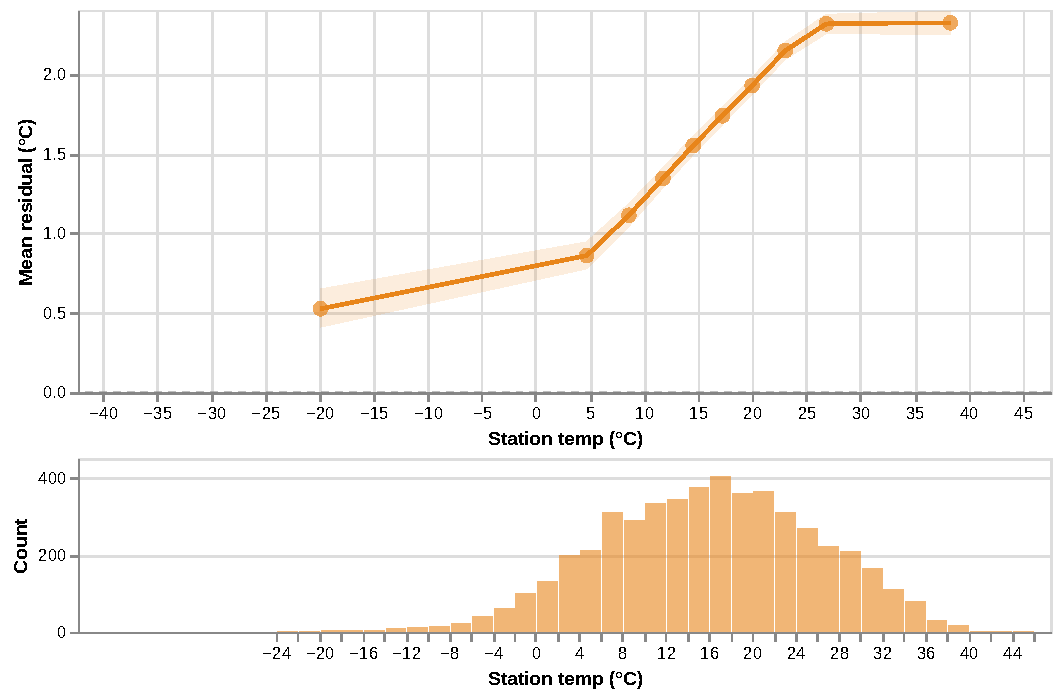
\includegraphics[width=\linewidth]{figures/pdp_station_celsius.pdf}
\caption{Station temperature}\label{fig:temperature}
\end{subfigure}%
\hfill
\begin{subfigure}[t]{0.32\textwidth}
\centering
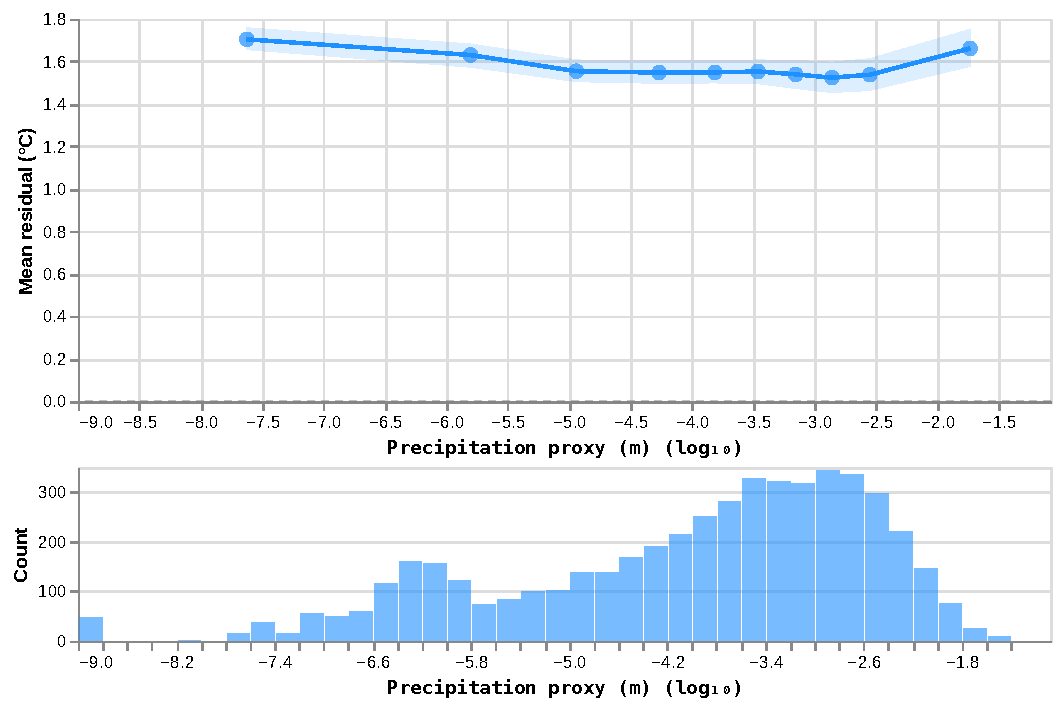
\includegraphics[width=\linewidth]{figures/pdp_tp.pdf}
\caption{Precipitation proxy}\label{fig:precip}
\end{subfigure}%
\hfill
\begin{subfigure}[t]{0.32\textwidth}
\centering
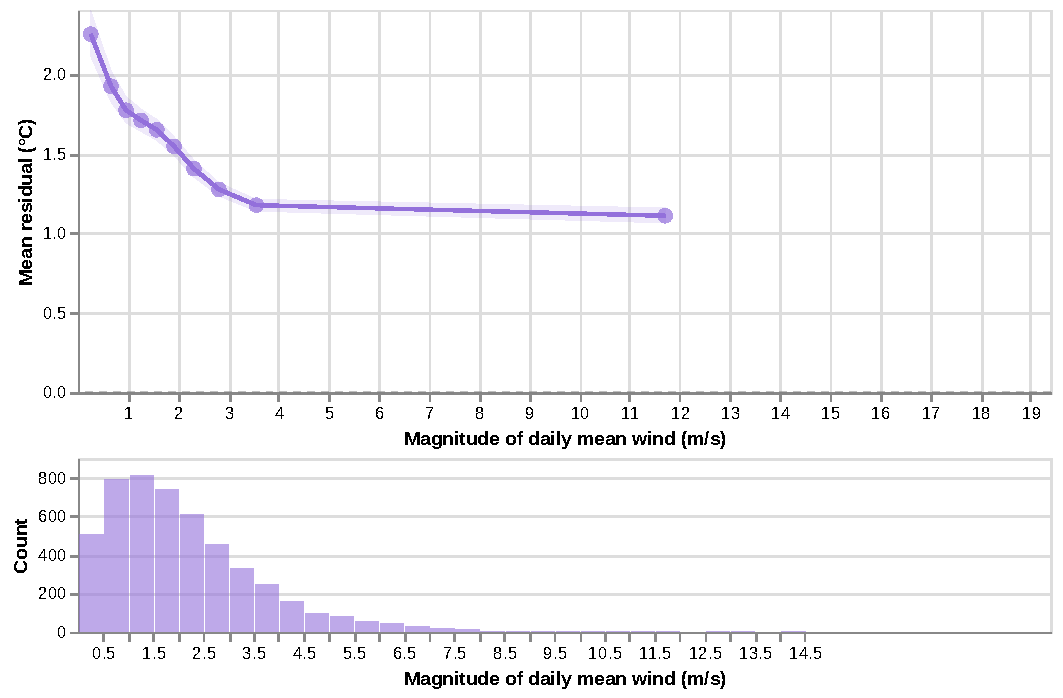
\includegraphics[width=\linewidth]{figures/pdp_wind.pdf}
\caption{Mean wind vector}\label{fig:wind}
\end{subfigure}%

\medskip

\begin{subfigure}[t]{0.32\textwidth}
\centering
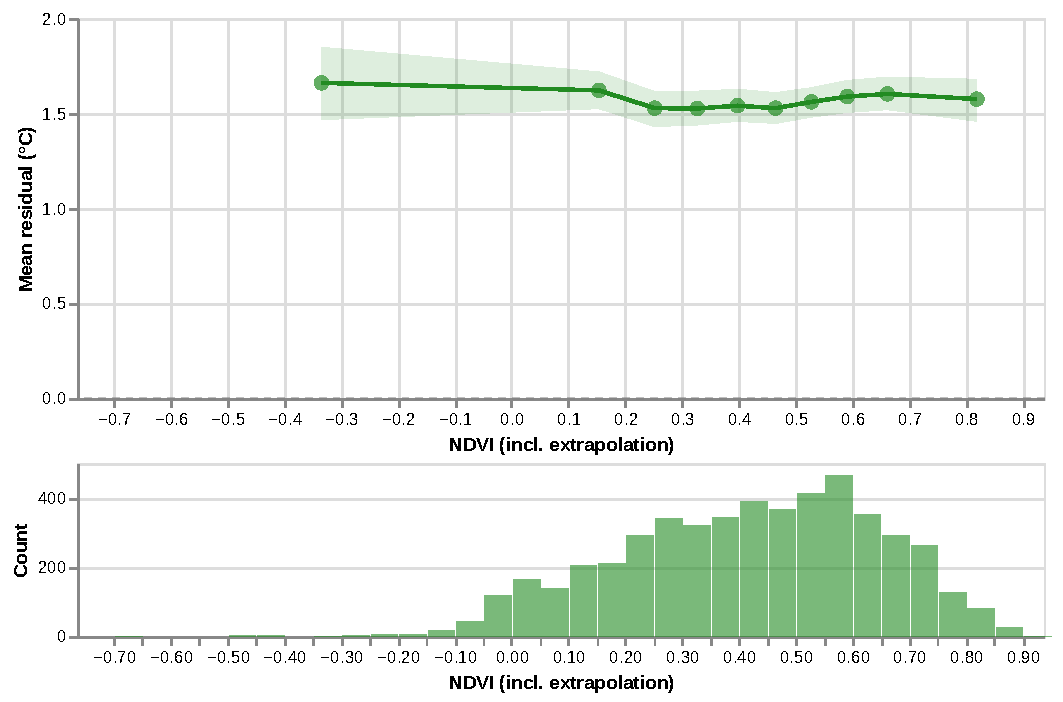
\includegraphics[width=\linewidth]{figures/pdp_ndvi.pdf}
\caption{NDVI}\label{fig:ndvi}
\end{subfigure}%
\hfill
\begin{subfigure}[t]{0.32\textwidth}
\centering
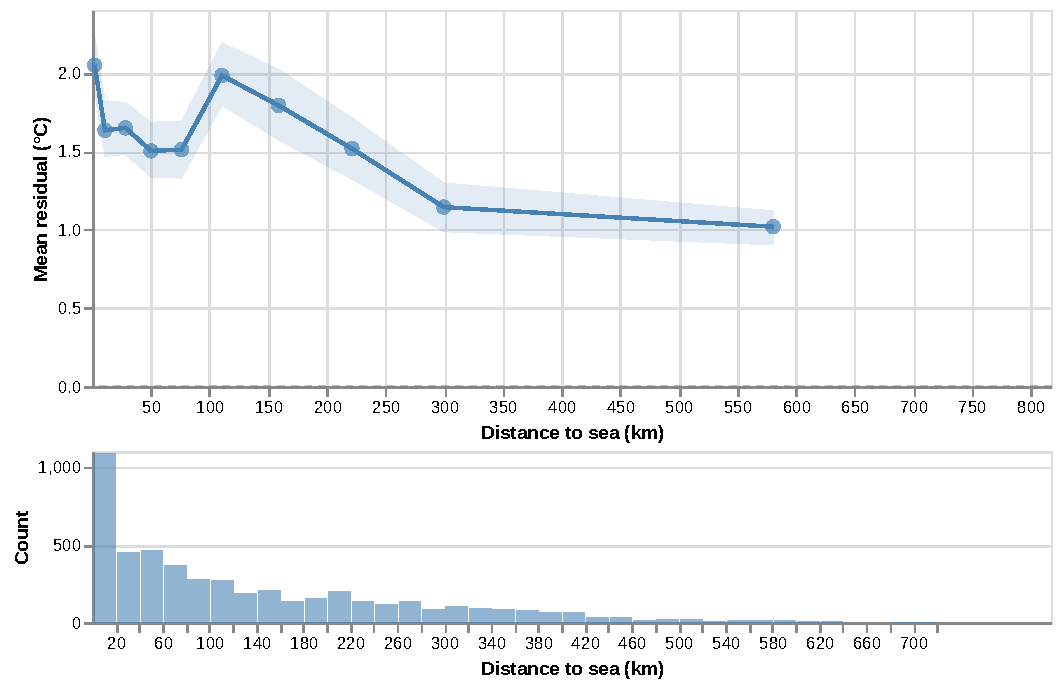
\includegraphics[width=\linewidth]{figures/pdp_dist_to_sea_km.pdf}
\caption{Distance to sea}\label{fig:coast}
\end{subfigure}%
\hfill
\begin{subfigure}[t]{0.32\textwidth}
\centering
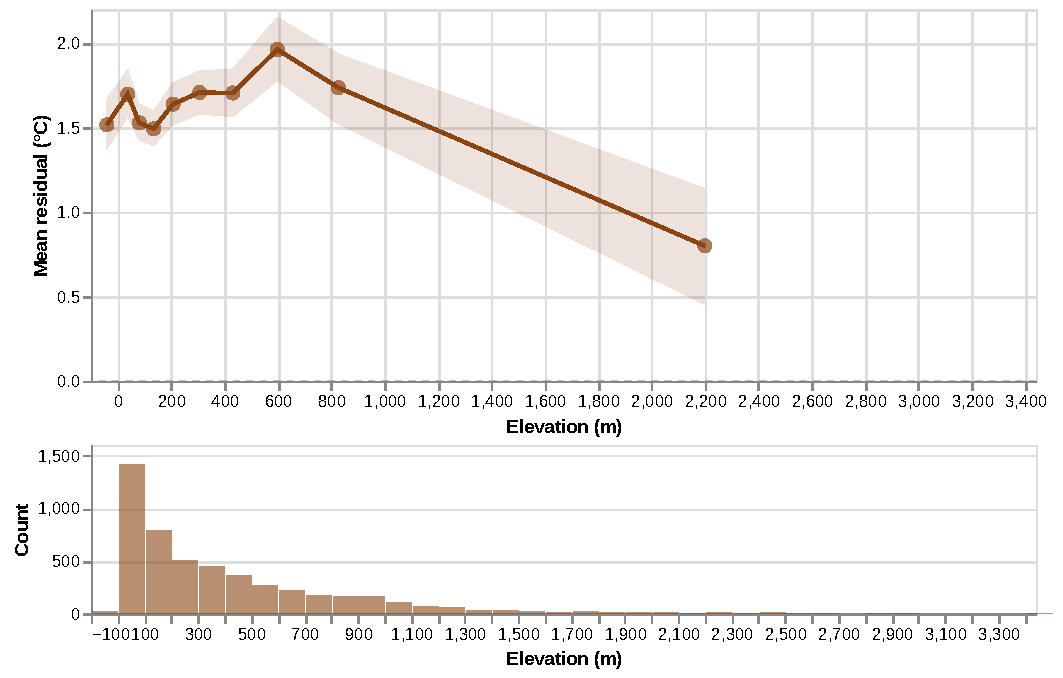
\includegraphics[width=\linewidth]{figures/pdp_elevation.pdf}
\caption{Elevation}\label{fig:elevation}
\end{subfigure}%
\caption{Mean residual by covariate quantile bin (upper panel of each subplot),
with pointwise 95\% station-bootstrap intervals. Lower histograms each use
4,999 sampled observations. Points mark bin midpoints. Precipitation is the
supplied proxy in metres, displayed as $\log_{10}(\max(\mathrm{tp},10^{-9}))$,
not a daily total. Wind is the magnitude of the daily mean vector. NDVI
includes flagged seasonal extrapolations; elevation excludes 3,825 missing
or invalid values. These are descriptive conditional means.}
\label{fig:pdp}
\end{figure}

Mean residual rises from $0.52\,^\circ$C in the lowest station-temperature
bin (maxima at or below $2.5\,^\circ$C) to $2.32\,^\circ$C in the highest
bin (above $29\,^\circ$C; Figure~\ref{fig:pdp}). The outer points represent
broad bins, not estimates at an individual extreme temperature. Station
temperature also enters the residual definition, so this marginal
association alone does not isolate a physical temperature effect.

\subsection{Smaller variations across precipitation-proxy and NDVI bins}
\label{sec:results-precip}

The precipitation-proxy bin means range from $1.52$ to $1.71\,^\circ$C
(Figure~\ref{fig:precip}). The pattern is not monotonic and cannot be
interpreted as a response to daily precipitation totals without resolving
the upstream accumulation convention.

NDVI bin means range from $1.53$ to $1.66\,^\circ$C, with substantially
overlapping pointwise intervals (Figure~\ref{fig:ndvi}). This is a small
descriptive variation; no formal test of no association is reported.
Interpretation also depends on the seasonal extrapolation policy.

\subsection{Residuals decrease across mean-vector wind bins}
\label{sec:results-wind}

The wind profile decreases across the displayed bins
(Figure~\ref{fig:wind}), from $2.25\,^\circ$C below approximately
$0.50\,\mathrm{m/s}$ to $1.11\,^\circ$C above approximately
$4.02\,\mathrm{m/s}$. This is a pooled association with mean-vector wind,
not a controlled estimate of the effect of atmospheric mixing.

\subsection{Distance to the sea and elevation}
\label{sec:results-geo}

The nearest-coast bin has mean residual $2.05\,^\circ$C, compared with
$1.02\,^\circ$C in the furthest-inland bin (above approximately 344 km).
The profile also has a secondary inland peak and is not monotonic
(Figure~\ref{fig:coast}).

The screened elevation profile is also non-monotonic
(Figure~\ref{fig:elevation}). Its largest bin mean is $1.96\,^\circ$C
between 500 and 695 m, falling to $0.80\,^\circ$C above 958 m.
It therefore does not support a simple increase in underestimation with
elevation. Station composition, terrain and source coverage may contribute
to both geographical profiles.

\subsection{Degree of urbanisation}
\label{sec:results-degurba}

\begin{figure}[htbp]
\centering
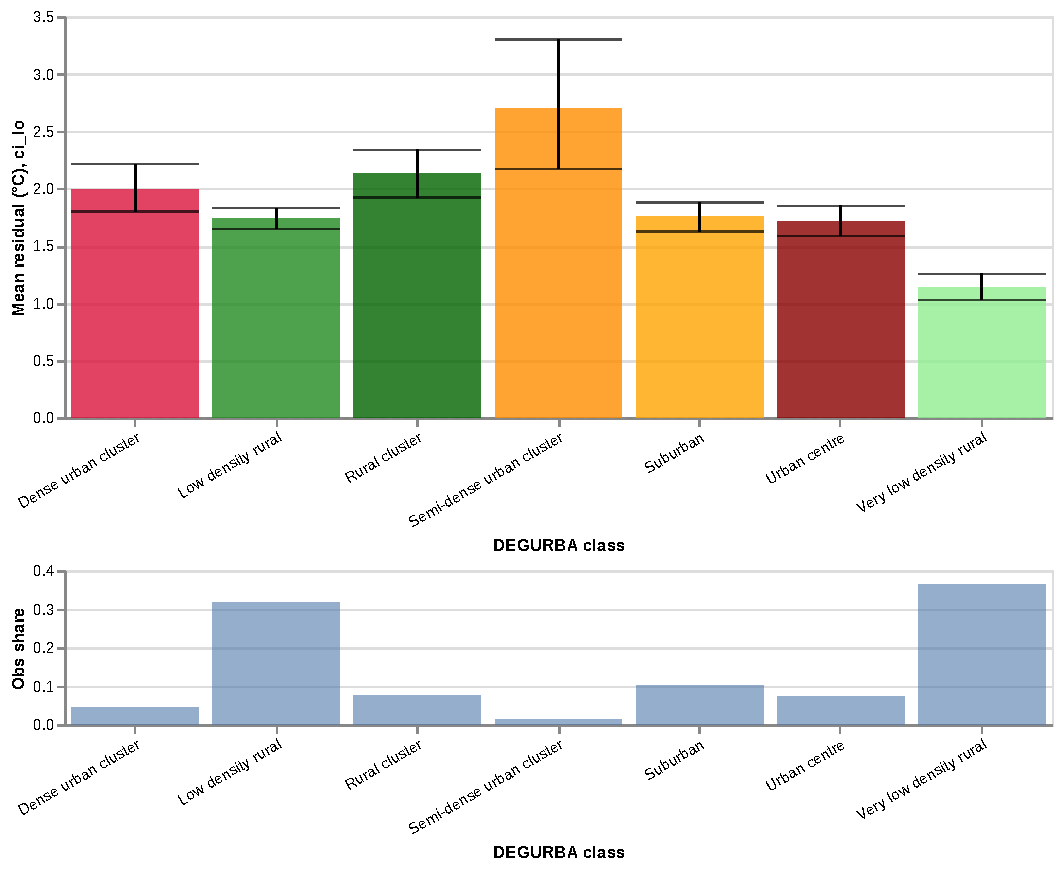
\includegraphics[width=\textwidth]{figures/degurba.pdf}
\caption{Mean residual for land DEGURBA classes (top), with
observation share of the full screened sample per land class (bottom).
Error bars are pointwise 95\% station-bootstrap intervals.
Water is omitted from both panels.}
\label{fig:degurba}
\end{figure}

Mean residual ranges from $1.14\,^\circ$C in very-low-density rural
locations to $2.70\,^\circ$C in semi-dense urban clusters; urban centres
average $1.72\,^\circ$C (Figure~\ref{fig:degurba}). The ordering is not
monotonic in urban density. The semi-dense class contains only 66 nominal
station IDs and has a comparatively wide interval. These class differences
cannot separate station siting, regional composition and unresolved urban
processes; they are not a direct estimate of an urban heat-island effect.

\subsection{The joint temperature$\times$wind profile}
\label{sec:results-interaction}

\begin{figure}[htbp]
\centering
\begin{subfigure}[t]{0.49\textwidth}
    \centering
    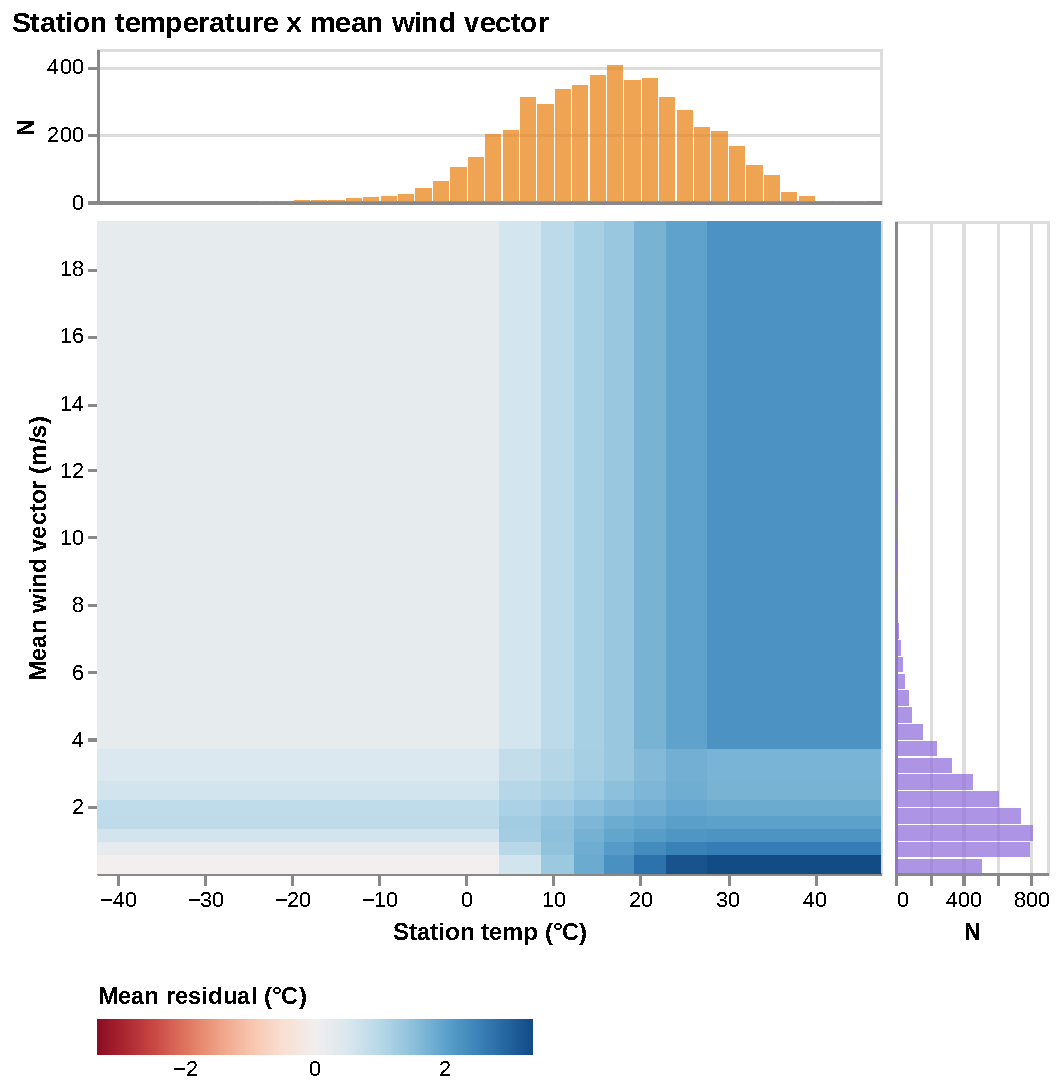
\includegraphics[width=\linewidth]{figures/station_celsius_by_wind.pdf}
    \caption{Station temperature $\times$ mean wind vector}
\end{subfigure}%
\hfill
\begin{subfigure}[t]{0.49\textwidth}
    \centering
    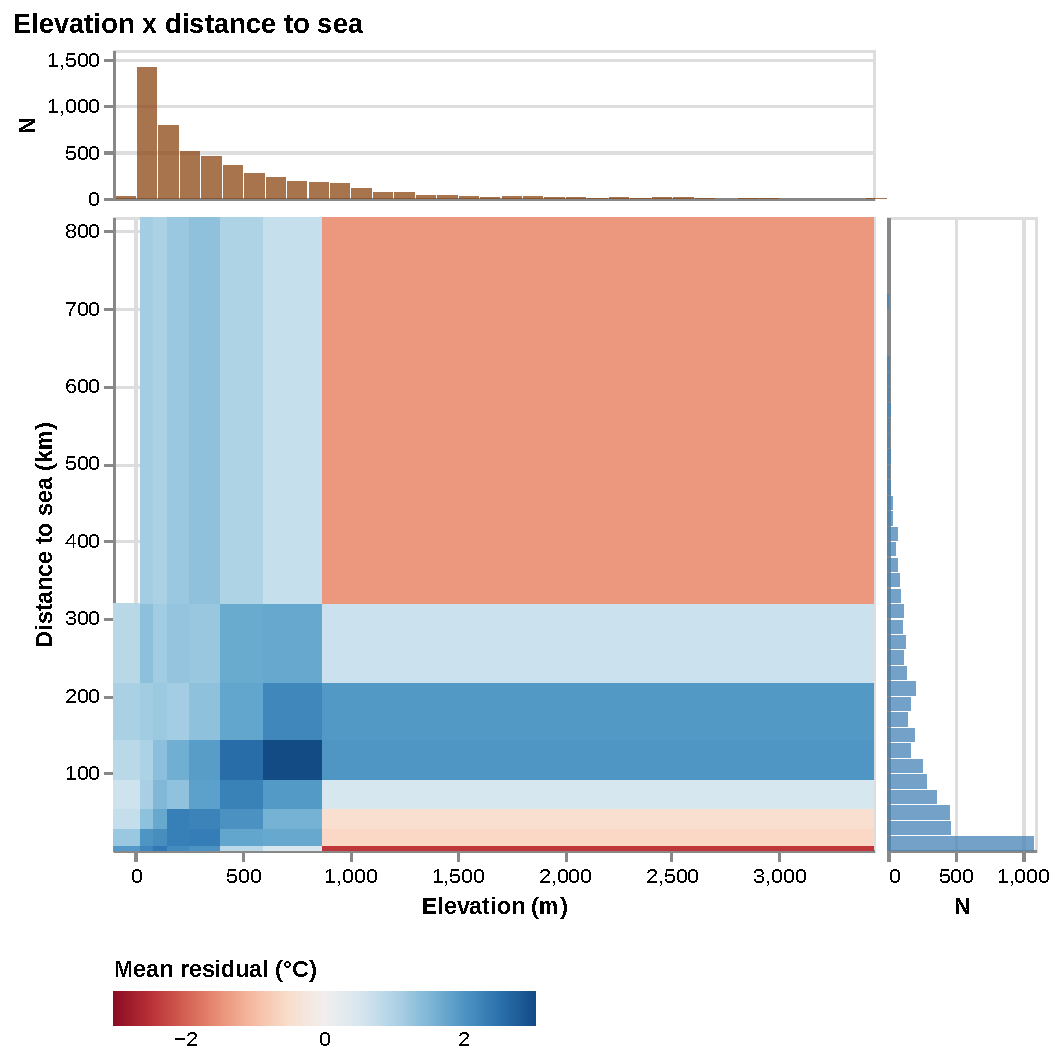
\includegraphics[width=\linewidth]{figures/elevation_by_dist_to_sea_km.pdf}
    \caption{Elevation $\times$ distance to sea}
\end{subfigure}
\caption{Observation-weighted mean residual in joint quantile bins
(eight bins per axis). Marginal histograms show 4,999 sampled observations
per axis. Each panel uses its own colour scale.
These are descriptive cell means; no confidence intervals are shown.}
\label{fig:interaction}
\end{figure}

The joint profile shows larger warm-temperature residuals under lower
mean-vector wind (Figure~\ref{fig:interaction}). In the warmest temperature
bin (above $27.7\,^\circ$C), mean residual is $3.36\,^\circ$C below
$0.58\,\mathrm{m/s}$, compared with $2.27\,^\circ$C above
$3.72\,\mathrm{m/s}$. These are different station-day groups, not a
within-station comparison or a formal interaction test. A boundary-layer
interpretation remains a hypothesis requiring additional controls.

\begin{table}[htbp]
\centering
\small
\caption{Descriptive ranges of the mean residual across the displayed bins or land classes. These ranges are not tests of statistical significance.}
\label{tab:results-summary}
\fitwidetable{%
\begin{tabular}{lrr}
\toprule
Covariate & Observed pattern & Range ($^\circ$C) \\
\midrule
Station temperature & Increasing & 0.52--2.32 \\
Mean wind vector & Decreasing & 1.11--2.25 \\
Distance to sea & Non-monotonic; lower inland & 1.02--2.05 \\
DEGURBA land classes & Non-monotonic across classes & 1.14--2.70 \\
Elevation & Non-monotonic & 0.80--1.96 \\
Precipitation proxy & Small variation & 1.52--1.71 \\
NDVI & Small variation & 1.53--1.66 \\
\bottomrule
\end{tabular}}
\end{table}


% ===========================================================================
\section{Discussion}
\label{sec:discussion}

\paragraph{Interpretation and threats to validity.}
The checks above establish consistency with the supplied source files,
but do not establish error-free station observations, physically identical
sampling intervals, or a representative sample of European land area.
The $1.58\,^\circ$C observation-weighted mean can reflect product error,
representativeness, observation windows and station selection. The
separate UTC subset addresses one aspect of the window mismatch; its
existence does not correct the mixed-window figures shown here.

The univariate and joint-bin profiles pool dates and stations and do not
control for the other covariates, seasonality or station composition.
Station temperature appears both as a predictor and in the residual
definition. A multivariate or within-station analysis would be needed
to distinguish conditional associations from these pooled relationships;
neither would by itself establish causality.

Bootstrap clusters are nominal station IDs. Source-day deduplication
removes repeated observations, but does not prove independence of physical
instruments or remove dependence between neighbouring stations. The
confidence intervals describe sampling variation under the stated
resampling scheme, not uncertainty from window mismatch, NDVI extrapolation,
screening choices or covariate measurement error. No formal multiplicity
adjustment, bin-difference test or joint interaction test is reported.

NDVI extrapolation assumes that a previous matching season is informative.
Recorded one- and two-year backtest mean absolute errors are approximately
0.073 and 0.071 NDVI units on 40,237 and 26,418 source-season comparisons,
respectively. The samples differ, so the smaller two-year error is not
evidence that longer extrapolation is preferable. Observed-only sensitivity
comparisons also change year and sample composition. Precipitation remains
a proxy, coast distance is approximate, and DEGURBA is fixed at 2020.
The temperature--wind pattern motivates a boundary-layer hypothesis,
but the present analysis does not identify that mechanism.

\paragraph{Consequences for downscaling.}
The descriptive profiles identify covariates and conditions worth testing
in future residual-based downscaling or bias-correction models. The joint
temperature--wind pattern suggests including dynamic as well as static
predictors, while the non-monotonic geographical profiles argue against
imposing a simple linear elevation or urban-density correction. These
diagnostics neither supply a validated correction model nor establish
where ERA5-Land can be treated as ground truth. Evaluation should preserve
separate training and validation samples and account for the sampling and
representativeness limitations identified here.

% ===========================================================================
\section{Conclusion}
\label{sec:conclusion}

Motivated by the GenHack'25 analyses, we compared ECA\&D daily maximum
temperatures with ERA5-Land daily maxima using a documented conservative
screening pipeline. In the retained sample, station maxima exceed the
reanalysis by $1.58\,^\circ$C on average when observations receive equal
weight. Conditional means increase across station-temperature bins and
decrease across mean-vector wind bins. Elevation, coastal-distance and
urban-class profiles are non-monotonic; NDVI and the precipitation proxy
show smaller descriptive ranges. The joint temperature--wind profile
is consistent with larger warm-temperature residuals under low mean-vector
wind, but does not establish a causal mechanism. Aligned-window sensitivity
analyses, validated screening rules, improved covariate provenance and
within-station or multivariate inference are needed before these patterns
can support a general European bias estimate or an operational correction.

\printbibliography

\end{document}
